% !TeX root = RJwrapper.tex
\title{\pkg{SurvMetrics}: An R package for Predictive Evaluation Metrics in Survival Analysis}
\author{by Hanpu Zhou, Hong Wang, Sizheng Wang and Yi Zou}

\maketitle

\abstract{
Recently, survival models have found vast applications in biostatistics, bioinformatics, reliability engineering, finance and related fields. But there are few R packages focusing on evaluating the predictive power of survival models. This lack of handy software on evaluating survival predictions  hinders further applications of survival analysis for practitioners. In this research, we want to fill this gap by providing an "all-in-one" R package which implements most predictive evaluation metrics in survival analysis. In the proposed \pkg{SurvMetrics} R package, we implement concordance index for both untied and tied survival data; we give a new calculation process of Brier score and integrated Brier score; we also extend the applicability of integrated absolute error and integrated square error for real data. For models that can output survival time predictions, a simplified metric called mean absolute error is also implemented. In addition, we test the effectiveness of all these metrics on simulated and real survival data sets.  The newly developed \pkg{SurvMetrics} R package is available on CRAN at \url{https://CRAN.R-project.org/package=SurvMetrics} and GitHub at \url{https://github.com/skyee1/SurvMetrics}.
}

\section{Introduction}

Survival analysis is an important part of biostatistics. It is frequently used to define prognostic indices for mortality or recurrence of a disease, and to study the outcome of treatment \citep{Wang.2019, Wijethilake.2021, fan.2016, wiens.2016}. Recent decades have witnessed many other applications of survival analysis in various disciplines such as finance, engineering and social sciences \citep{Steyerberg.2010, Bender.2020, Wang.2019}. Evaluating the ability to predict future data is one of the most important considerations in the development of these survival models \citep{Wang.2019}.

\begin{figure}[h]
\centering
\begin{center}
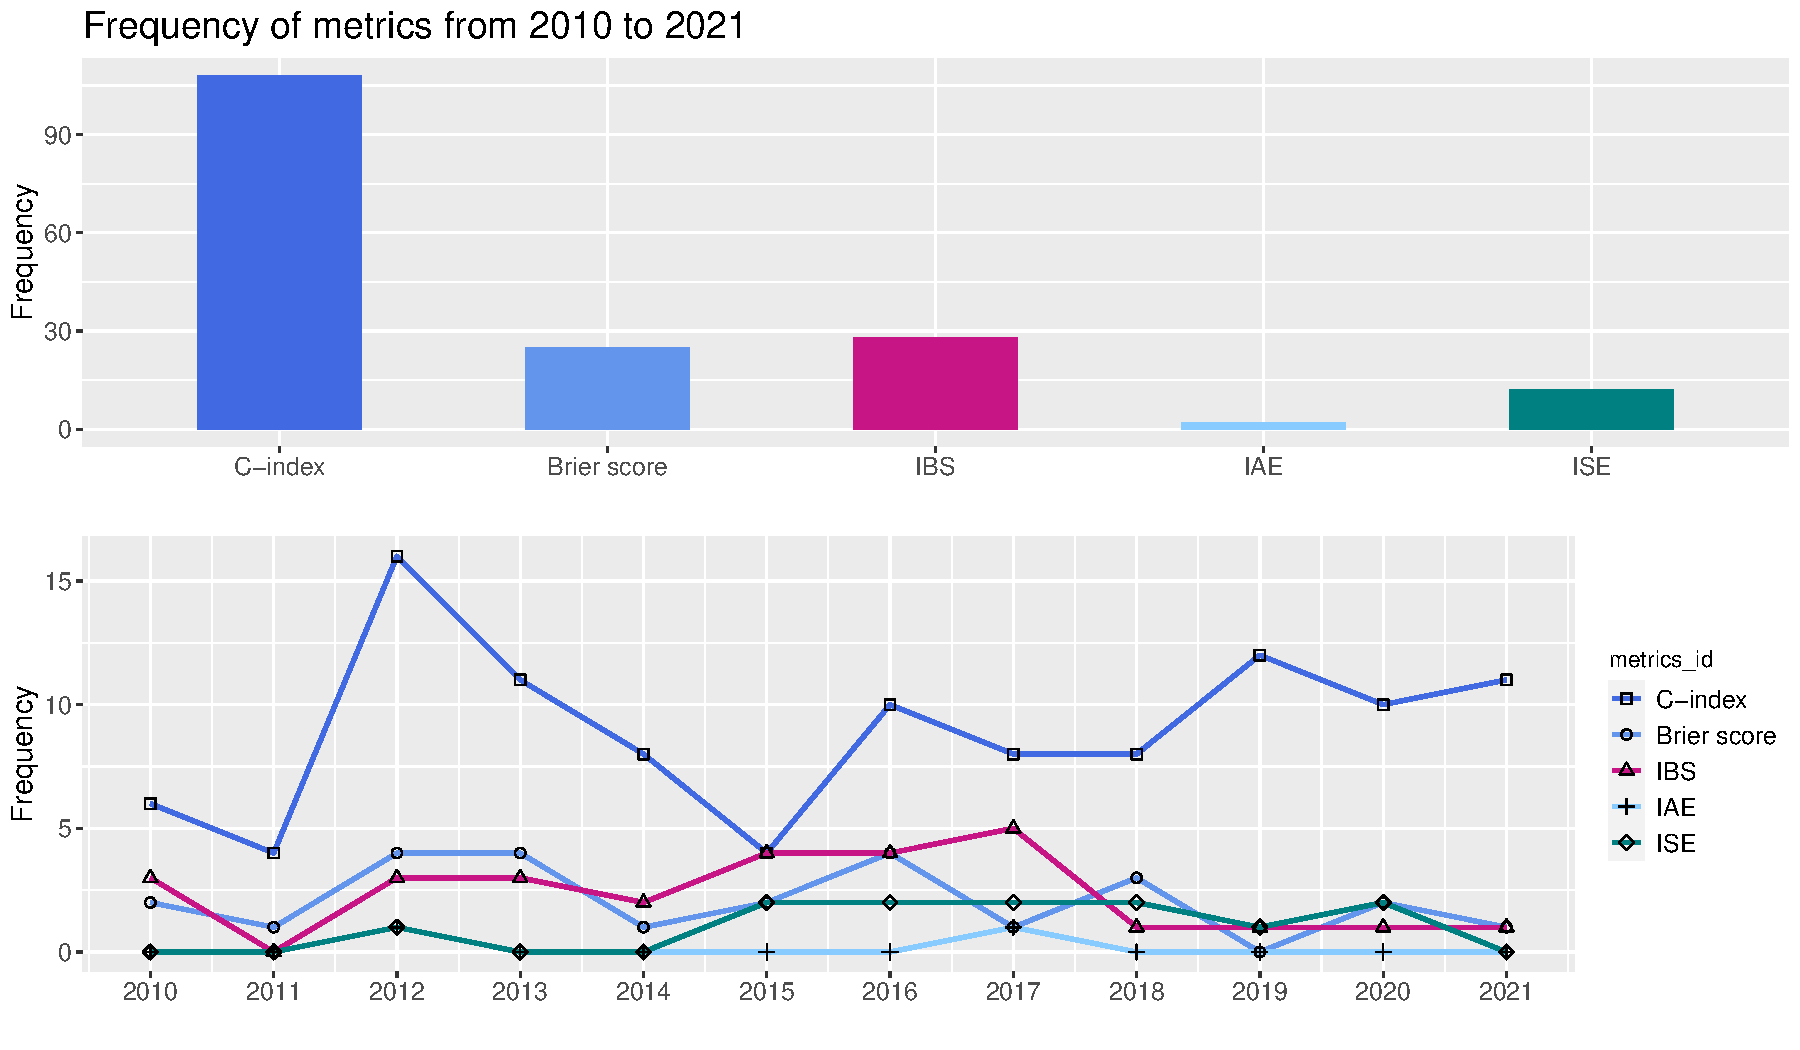
\includegraphics[width=\textwidth]{bothbarline.pdf}
\caption{
Frequency of survival model evaluation metrics appearing in journals such as "\emph{Annals of Statistics}", "\emph{Biometrika}", "\emph{Journal of the American Statistical Association}", "\emph{Journal of the Royal Statistical Society, Series B}", "\emph{Statistics in Medicine", "Artificial Intelligence in Medicine}", "\emph{Lifetime Data Analysis}" from 2010 to 2021.}\label{figbarline}
\end{center}
\end{figure}

When evaluating a prediction model, the predictive performance of the survival model is commonly addressed by appropriate measures which quantify the 'distance' or the agreement between the observed and predicted outcomes \citep{uno.2011, bylinskii.2018}. By investigating the predictive measures frequently used in the statistical literature (top or specialized statistical journals) in the past decade (from 2010 to 2021) in Figure \ref{figbarline} and Figure \ref{figpie}, we have found that among these 136 research papers, the popular predictive metrics for survival models mainly include: concordance index (C-index), Brier score (BS), integrated Brier score (IBS), integrated absolute error (IAE), integrated square error (ISE) and mean absolute error (MAE) \citep{Harrell.1982, Brier.1950, Graf.1999, Hoora.2017, Schemper.1992}.


\begin{figure}[h]
\centering
\begin{center}
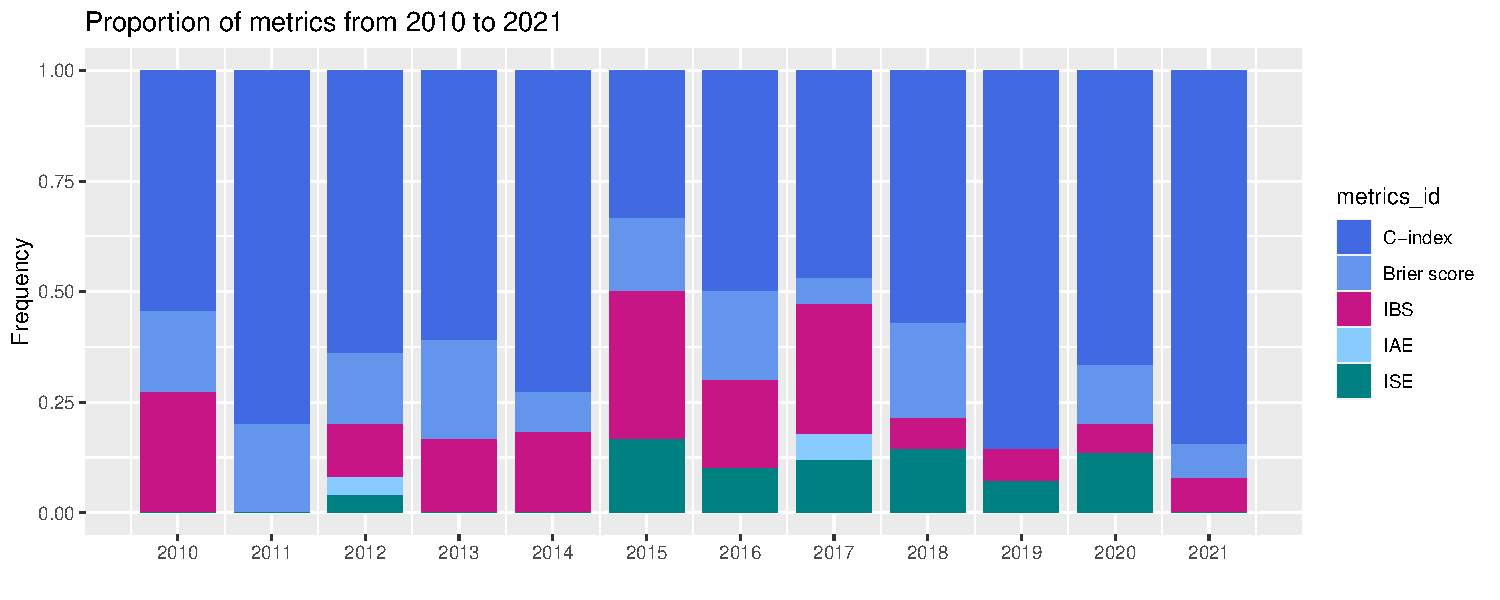
\includegraphics[width=\textwidth]{pie.pdf}
\caption{
This graphic shows the percentage of metrics appearing from 2010 to 2021 in journals such as "\emph{Annals of Statistics}", "\emph{Biometrika}", "\emph{Journal of the American Statistical Association}", "\emph{Journal of the Royal Statistical Society, Series B}", "\emph{Statistics in Medicine", "Artificial Intelligence in Medicine}", "\emph{Lifetime Data Analysis}". It indicates that the use of C-index is steadily increasing and it has become a dominant predictive measure recently. Meanwhile, other metrics do not have an adequate seat in survival prediction practices.}\label{figpie}
\end{center}
\end{figure}

From Figure \ref{figbarline}, we can see that the two most frequently used metrics are C-index and IBS, while the other metrics are less used. This may be partly due to the fact that the available predictive metrics are scattered across several R packages, and differences in input data of these tools make it difficult for non-specialists to use or compare the survival models \citep{survcomp.2011, ipred.2009}. Hence, software which provides easy input data formats and includes most popular metrics is desirable \citep{survcomp.2011, Wang.2019}.

Figure \ref{figpie} indicates that the use of C-index is steadily increasing and it has become a dominant predictive measure recently \citep{Jing.2019, Amico.2021}. On the one hand, this implies that the lack of handy evaluation metrics tools since other measures are also very important in survival analysis but do not have an adequate seat in survival prediction practices \citep{Nemati.2021, Li.2021, ensor.2021}. On the other hand, it reminds us that providing an accurate C-index measure which can take various situations into account is extremely important \citep{HEaGerty.2005, Kang.2015, zadeh.2020, zhang.2021}.

Different from common classification or regression problems where tools to evaluate predictive performance are abundant, there are few R packages focusing on evaluating the predictive power of survival models \citep{Hmisc.2019, ipred.2009}. To make things worse, most of these available packages have implemented only one or two evaluation metrics and/or some of them often throw errors in real survival problems \citep{ipred.2009}. Take the C-index for an example, if the user wants to compare two samples with the same survival time, this scenario returns NA in \pkg{Hmisc}, \pkg{survivals}, and \pkg{survcomp} packages. However, as described by \cite{Ishwaran.2008}, "for sample pairs, where observed time $X_i = X_j$ and both are deaths, count 1 if predicted outcomes are tied." This error is mainly due to the fact that the above packages ignore this possible scenario in practice. Omitting such scenarios can result in the loss of information from survival data, especially when the sample size is small with high data collection costs. In \pkg{SurvMetrics}, we have implemented the method described by \cite{Ishwaran.2008} to cover all tied scenarios.
%For example, in the \pkg{Hmisc} and \pkg{survival} packages, the calculation of C-index could be an issue if tied data are present \citep{Harrell.1996, Hmisc.2019}.
There are also functions available in the \pkg{ipred} package to calculate BS and IBS values, but a list of \dfn{survfit} objects is required in the calculation process \citep{ipred.2009}. However, for most survival models, only a survival probability vector or matrix is provided, making calculations of such values a challenging problem \citep{Ishwaran.2008}. It is not easy for non-specialists to get IBS using the \pkg{ipred} package directly on the survival model results.

We argue that an appealing survival evaluation metric tool should satisfy the following two properties. First, the evaluation metrics should not depend on any specific model and they can be applied to evaluating survival models without specifying a specific model form \citep{survcomp.2011}. Second, the metrics should be computationally tractable and user has the choice to input only the fitted model without any additional processing, especially for the non-specialist  \citep{Harrell.1982, Graf.1999, Hoora.2017, Ishwaran.2008}.

In this research, we are trying to develop a comprehensive and effective R package with the above two properties. In the proposed \pkg{SurvMetrics} package, the calculation process of most metrics does not depend on the specific model form and only predicted survival probability vector (or matrix) is needed. This feature is particularly desirable for non-statistical researchers such as clinical and financial practitioners \citep{ali.2021}. To illustrate the effectiveness of our tool, we choose two popular survival models, namely, a semi-parametric Cox model and a non-parametric random survival forest model (RSF) to check and test the provided functionalities \citep{cox.1972, Ishwaran.2008}.

\section{Predictive evaluation metrics in survival analysis}

In this section, we will present the survival model evaluation metrics and some implementing details. The following Table \ref{tab1} presents some popular R packages and the metrics they provide.

\begin{table}[h]
\centering
\begin{tabular}{lcccccc}
\hline
\textbf{Packages}    & C-index & BS &IBS &IAE &ISE &MAE \\
\hline
\pkg{survival}    & \Checkmark   & \XSolidBrush & \XSolidBrush & \XSolidBrush & \XSolidBrush  & \XSolidBrush    \\
\pkg{Hmisc} & \Checkmark   & \XSolidBrush & \XSolidBrush & \XSolidBrush & \XSolidBrush  & \XSolidBrush    \\
\pkg{survcomp}    & \Checkmark   & \Checkmark  & \Checkmark  & \XSolidBrush & \XSolidBrush  & \XSolidBrush    \\
\pkg{ipred}       & \XSolidBrush  & \Checkmark  & \Checkmark  & \XSolidBrush & \XSolidBrush  & \XSolidBrush    \\
\pkg{mlr}       & \XSolidBrush  & \XSolidBrush  & \XSolidBrush  & \XSolidBrush & \XSolidBrush  & \Checkmark    \\
\pkg{SurvMetrics} & \Checkmark   & \Checkmark  & \Checkmark  & \Checkmark  & \Checkmark   & \Checkmark\\
\hline
\end{tabular}
\caption{
R packages that are commonly used to evaluate survival predictions. }
	\label{tab1}
\end{table}


As can be seen in Table \ref{tab1}, the proposed \pkg{SurvMetrics} package implements all popular evaluation metrics, while other packages mostly implement just one or two. With our \pkg{SurvMetrics} package, one can compare and evaluate different survival models in a convenient and comprehensive way.

\subsection{C-index}

The most popular evaluation metric in survival predictions is C-index \citep{Harrell.1982, Li.2016, Lee.2018, Devlin.2021, subramanian.2020, hsu.2020, zadeh.2020, zhang.2021, Wanghong.2017, Wanghong.2019}, which is a generalization of the ROC curve \citep{HEaGerty.2005, Obuchowski.2006, Kang.2015, Li.2016}.
C-index intends to measure the proportion of predictions of the binary survival status that agree with the true survival status. If the study is concerned with the comparison of survival probability between different samples, for example, which component in the device shows damage earlier, the C-index can be used.

To calculate the values of C-index from different models, \pkg{Hmisc}, \pkg{survcomp} and \pkg{survival} R packages are frequently used in practice \citep{Harrell.1996, survcomp.2011, survival.2014, Hmisc.2019}. All the above-mentioned packages in their current versions do not consider the cases of tied survival data, i.e., samples with the same survival time. As shown in Table \ref{tab3-1res}, they return 0 or NA for all cases of survival data tied. However, in practice, cancer patients are usually surveyed annually or monthly after surgery for survival status and with the advent of big data, tied samples are becoming commonplace. Simply ignoring the presence of tie data in calculating C-index will result in evaluation bias among survival models.

Meanwhile, in the calculation of the C-index, not all sample pairs are comparable, e.g., for those pairs whose shorter survival time is censored. So it is necessary to filter the sample pairs $(i, j)$ that can be compared in the calculation, i and j denote any two samples in the data set, respectively. By defining the comparable sample pair in the following way, when $np_{ij} = 1$, all comparable sample pairs described by \cite{Ishwaran.2008} can be covered.

In the proposed R package, we will take a similar strategy adopted in \cite{Ishwaran.2008}. $\delta_i$ denotes the survival status of sample $i$ (0 means censoring, 1 means event), $Y_i$ and $X_i$ represent the predicted survival time and the observed survival time, respectively. By defining $csign$ and $sign$, we can easily distinguish which sample pairs meet the concordance and which are not.


\begin{enumerate}[label=(\alph*)]
  \item The comparable sample pair is defined as:
\begin{equation}\label{compairs}
  np_{ij}\left(X_{i}, \delta_{i}, X_{j}, \delta_{j}\right) = \max(I\left(X_{i} \geqslant X_{j}\right) \delta_{j},I\left(X_{i} \leqslant X_{j}\right) \delta_{i}).
\end{equation}
  \item The complete concordance (CC) is defined as:
\begin{equation}\label{CC}
  \text{CC} = \sum_{i,j}I({\rm sign}(Y_i,Y_j)={\rm csign}(X_i,X_j)|np_{ij}=1),
\end{equation}
where
\begin{equation}\label{sign}
  {\rm sign}(Y_i,Y_j) = I\left(Y_{i} \geqslant Y_{j}\right) -I\left(Y_{i} \leqslant Y_{j}\right)
\end{equation}
and
\begin{equation}\label{csign}
  {\rm csign}(X_{i}, \delta_{i}, X_{j}, \delta_{j})=I(X_{i} \geqslant X_{j}) \delta_{j}-I\left(X_{i} \leqslant X_{j}\right) \delta_{i}.
\end{equation}
  \item We derive the partial concordance (PC):
\begin{equation}\label{PC}
\begin{aligned}
\text{PC} &=\sum_{i, j} I\left(Y_{i}=Y_{j} \mid n p_{i j}=1, X_{i} \neq X_{j}\right) \\
&+I\left(Y_{i} \neq Y_{j} \mid n p_{i j}=1, X_{i}=X_{j}, \delta_{i}=\delta_{j}=1\right) \\
&+I\left(Y_{i} \geq Y_{j} \mid n p_{i j}=1, X_{i}=X_{j}, \delta_{i}=1, \delta_{j}=0\right).
\end{aligned}
\end{equation}
  \item The C-index value can be given by:
\begin{equation}\label{CI}
  C\text{-}index =\frac{\text{concordance}}{\text{permissible}} = \frac{CC+0.5\times PC}{\sum_{i,j}np_{ij}(X_i,\delta_i,X_j,\delta_j)},
\end{equation}
\end{enumerate}


From the above, we know C-index lies between 0 and 1 and usually the larger the C-index, the more accurate prediction the model can get.

To further illustrate the proposed \code{Cindex()} function in \pkg{SurvMetrics} with other packages, we first give a toy example in Table \ref{tab3-1data}.

\begin{table}[!ht]
\centering
\begin{tabular}{lcccccccc}
\hline
\textbf{sample} & $S_1$  & $S_2$  & $S_3$  & $S_4$  & $S_5$  & $S_6$  & $S_7$  & $S_8$  \\ \hline
\textsf{time}      & 1   & 1   & 2   & 2   & 2   & 2   & 2   & 2   \\

\textsf{status}    & 0   & 1   & 1   & 0   & 1   & 1   & 0   & 1   \\

\textsf{predicted} & 0.2 & 0.3 & 0.3 & 0.3 & 0.4 & 0.2 & 0.4 & 0.3\\
\hline
\end{tabular}
\caption{
\noindent A simulation data set which can include all the possible sample pairs, where \textsf{time} and \textsf{status} are the observed survival time and survival status of samples $S_1...S_8$, respectively, and \textsf{predicted} is the survival probability predicted by survival models.}\label{tab3-1data}
\end{table}

Based on the above information, different R packages will take different ways to deal with these predictions. We summarize these calculation differences behind these R packages in Table \ref{tab3-1res}.

\begin{table}[!ht]
  \centering
  \resizebox{\textwidth}{!}{
  \begin{tabular}{lcccccccc}
    \hline
    \textbf{sample pair} & $(S_1, S_2)$ & $(S_3, S_5)$ & $(S_3, S_6)$ & $(S_3, S_8)$ & $(S_4, S_5)$ & $(S_5, S_6)$ & $(S_5, S_8)$ & $(S_6, S_8)$ \\ \hline
    \pkg{Hmisc}    & 0 & NA & NA & NA & 0 & NA & NA & NA \\
    \pkg{survival} & 0 & NA & NA & NA & 0 & NA & NA & NA \\
    \pkg{survcomp} & NA & NA & NA & NA & NA & NA & NA & NA \\
    \pkg{SurvMetrics} & 0.5 & 0.5 & 0.5 & 1 & 0.5 & 0.5 & 0.5 & 0.5 \\
    \hline
  \end{tabular}
  }
\caption{
Differences of C-index calculated by the \pkg{Hmisc} package, the \pkg{survival} package, the \pkg{survcomp} package and the \pkg{SurvMetrics} package.}\label{tab3-1res}
\end{table}

From the above, we can find that when ignoring part or all of the information from tied sample pairs, the C-index values obtained from \pkg{Hmisc} and other two packages cannot reflect the predictive powers of survival models in a true manner. In this case, one can turn to the \code{Cindex()} function in \pkg{SurvMetrics} package for help.

\subsection{BS}

BS is another commonly used metric in survival analysis \citep{Steyerberg.2010, chicco.2021, imani.2019, pakbin.2018}, which measures the mean squared error between the observed progression status and the predicted survival probability at time $t^*$. Thus, a lower BS usually indicates a better prediction model. BS focuses on the residuals between the predicted survival probability and the survival status at a fixed time point. If the study is concerned with the prediction probability of a model at a fixed time point, BS can be chosen as the metric. For example, the 10-year average survival probability of cancer patients.

In the \pkg{SurvMetrics} R package we will take the most classical method to calculate the BS by weighting the prediction residuals with inverse probability censoring weights (IPCW) proposed by \cite{Graf.1999}:

\begin{equation}\label{BS}
BS(t^*)=\frac{1}{N}\sum_{i=1}^N\left[\frac{(\hat{S}(t^*|z_i))^2}{\hat{G}(X_i)}\cdot I(X_i<t^*,\delta_i=1)+\frac{(1-\hat{S}(t^*|z_i))^2}{\hat{G}(t^*)}\cdot I(X_i\ge t^*)\right],
\end{equation}
where $t^*$ is the time point at which BS is to be calculated, $N$ is the sample size, $z_i$ is the covariates of instance $i$, $\hat{S}(\cdot)$ is the survival function predicted by the model, $\hat{G}(\cdot)$ denotes the weight for the instance which is estimated by the KM(Kaplan–Meier) estimator of the censoring distribution.

According to the definition of BS, its value depends on the selection of $t^*$ provided by the user and different choices of $t^*$ will always lead to different BS values \citep{Chew.2001, Li.2021, Zhu.2012, Ji.2020}. In the \code{Brier()} function of our \pkg{SurvMetrics} R package, $t^*$ is set to median survival time as default.



\subsection{IBS}

As we can see above, BS depends partly on the choices of a user-specified time point. It makes the comparison between models somewhat difficult when we want to know an average prediction performance over all prediction times. In practice, the integral of BS or IBS, which does not depend on the selection of one time point, is more widely used when we are interested in the entire time interval \citep{Zhu.2012, perianez.2016, bertens.2017}. IBS is more concerned with the residuals at all observed time points. When the time of interest is no longer a specific time point, IBS can provide more information than BS. For example, the probability of survival of a cancer patient for each year after the disease.

The definition of IBS is straightforward:

\begin{equation}\label{IBS}
  IBS=\frac{1}{\max\limits_i{(X_i)}} \int_0^{\max\limits_i(X_i)}BS(t)dt.
\end{equation}

But the calculation of IBS using \code{sbrier()} function from the \pkg{ipred} package does not always go smoothly \citep{ipred.2009} . If a list of \code{survfit} objects is incorrectly specified, then the package currently returns a particular error:

\samp{Error in switch(ptype, survfit = \{ : EXPR must be a length 1 vector\} }

In our experience, this kind of error is common, especially for the non-specialists \citep{ipred.2009}.

In the \pkg{SurvMetrics} package,  we will make life easier for non-specialists.  Users only need to input survival time, survival status, the predicted survival probability matrix and the range of integration to the \code{IBS()} function, and our program will take care of all the rest work and give a correct output. Similar to BS, a smaller IBS value usually implies a more accurate survival model.

\subsection{IAE and ISE}

Another two evaluation metrics, namely, IAE and ISE are also occasionally used to compare the difference between the estimated survival function $\hat{S}(\cdot)$ and the true survival function $S(\cdot)$ in terms of $L_1$ and $L_2$ paradigms, respectively. When the purpose of the model is to approximate the theoretical distribution function, IAE and ISE can be selected as the metrics. \cite{Hoora.2017, Zou.2021}.  The IAE and ISE can be defined as:

\begin{equation}\label{IAE}
  IAE=\int_{t}|S(t)-\hat{S}(t|X)| dt
\end{equation}
and
\begin{equation}\label{ISE}
  ISE =\int_{t}(S(t)-\hat{S}(t|X))^{2} dt,
\end{equation}
where $X$ is the covariate of the training set.

Since the true survival functions are usually unknown beforehand, traditional IAE and ISE methods are only applicable to simulation scenarios.  Here, we propose to approximate $S(t)$ using the non-parametric KM estimator in the \code{IAEISE()} function and this makes IAE and ISE also suitable for real data study. Similar to IBS, a smaller IAE and ISE values lead to a more accurate model.


\subsection{MAE}

The last evaluation metric presented here is MAE \citep{Schemper.1992}, which can be used to measure the residuals of observed survival time versus predicted survival time, for example, to predict the time to damage of the device. MAE is a better choice than BS if predicted survival time is a model's output. The definition of MAE is shown below:


    \begin{equation}\label{MAE}
  MAE=\frac{1}{n} \sum_{i=1}^{N}\left(\delta_{i}\left|Y_{i}-{X}_{i}\right|\right),
  \end{equation}

  \noindent where $n$ is the event sample size.

MAE only estimates the average absolute error between the predicted survival time and the true survival time in the uncensored samples and is rarely used in practice. For consistence, we also provide this metric in the \code{MAE()} function. Similar to MSE, the lower the MAE, the higher the accuracy of prediction.


\section{Simulations and examples}\label{sec3}

In this section, we will use some simulated and real survival data sets to illustrate the effectiveness of the metrics provided in the \pkg{SurvMetrics} package.

\subsection{The performance of \pkg{SurvMetrics} on simulation data sets}\label{sec3.1}

First, Cox proportional hazard models will be fitted on three simulated scenarios which are very similar to Settings 1–4 by \cite{Steingrimsson.2019}. Scenario1 satisfies the proportional hazards assumption and others violate it.
%Theoretically, the prediction performance of the Cox model should become worse and worse with increased violation of the proportional hazards assumption.

\begin{sloppypar}

  \noindent \textbf{Scenario1:}
  This data set is created using $N$ independent observations, where the covariate vector ($ W_1, . . . ,W_{p} $) is multivariate normal with mean zero and a covariance matrix having elements $(i, j)$ equal to $0.9^{|i-j|}$. Survival times are simulated from an exponential distribution with mean $ \mu = e^{0.1 \sum_{i=[p/2]+1}^{p}W_i} $ (i.e., a proportional hazards model) and the censoring distribution is exponential with mean $c_{mean}$ which is chosen to control the censoring rate. Here, $[x]$ denotes the largest integer no more than x.

  \noindent \textbf{Scenario2:}
  This data set is created using $N$ independent observations where the covariates ($W_1, . . . ,W_{p}$) are multivariate normal with mean zero and a covariance matrix having elements $(i, j)$ equal to $0.75^{|i-j|}$. Survival times are gamma distributed with shape parameter $\mu = 0.5 + 0.3\lvert\sum_{i=[2p/5]}^{[3p/5]} W_i\rvert $ and scale parameter 2. Censoring times are uniform on $[0, u_{max}]$, and $u_{max}$ is chosen to control the censoring rate. Here, the proportional hazards assumption is violated.

  \noindent \textbf{Scenario3:}
  This data set is created using $N$ independent observations where the covariates $(W_1, . . . ,W_{p})$ are multivariate normal with mean zero and a covariance matrix having elements $(i, j)$ equal to $0.75^{|i-j|}$. Survival times are simulated according to a log-normal distribution with mean $\mu = 0.1\lvert \sum_{i=1}^{[p/5]} W_i\rvert + 0.1\lvert\sum_{i=[4p/5]}^{p}W_i\rvert$. Censoring times are log-normal with mean $ \mu + c_{step} $ and scale parameter one, where $c_{step}$ is chosen to control the censoring rate. Here, the underlying censoring distribution depends on covariates and the proportional hazards assumption is also violated.
  \end{sloppypar}

\begin{figure}[h]
  \centering
  \begin{center}
  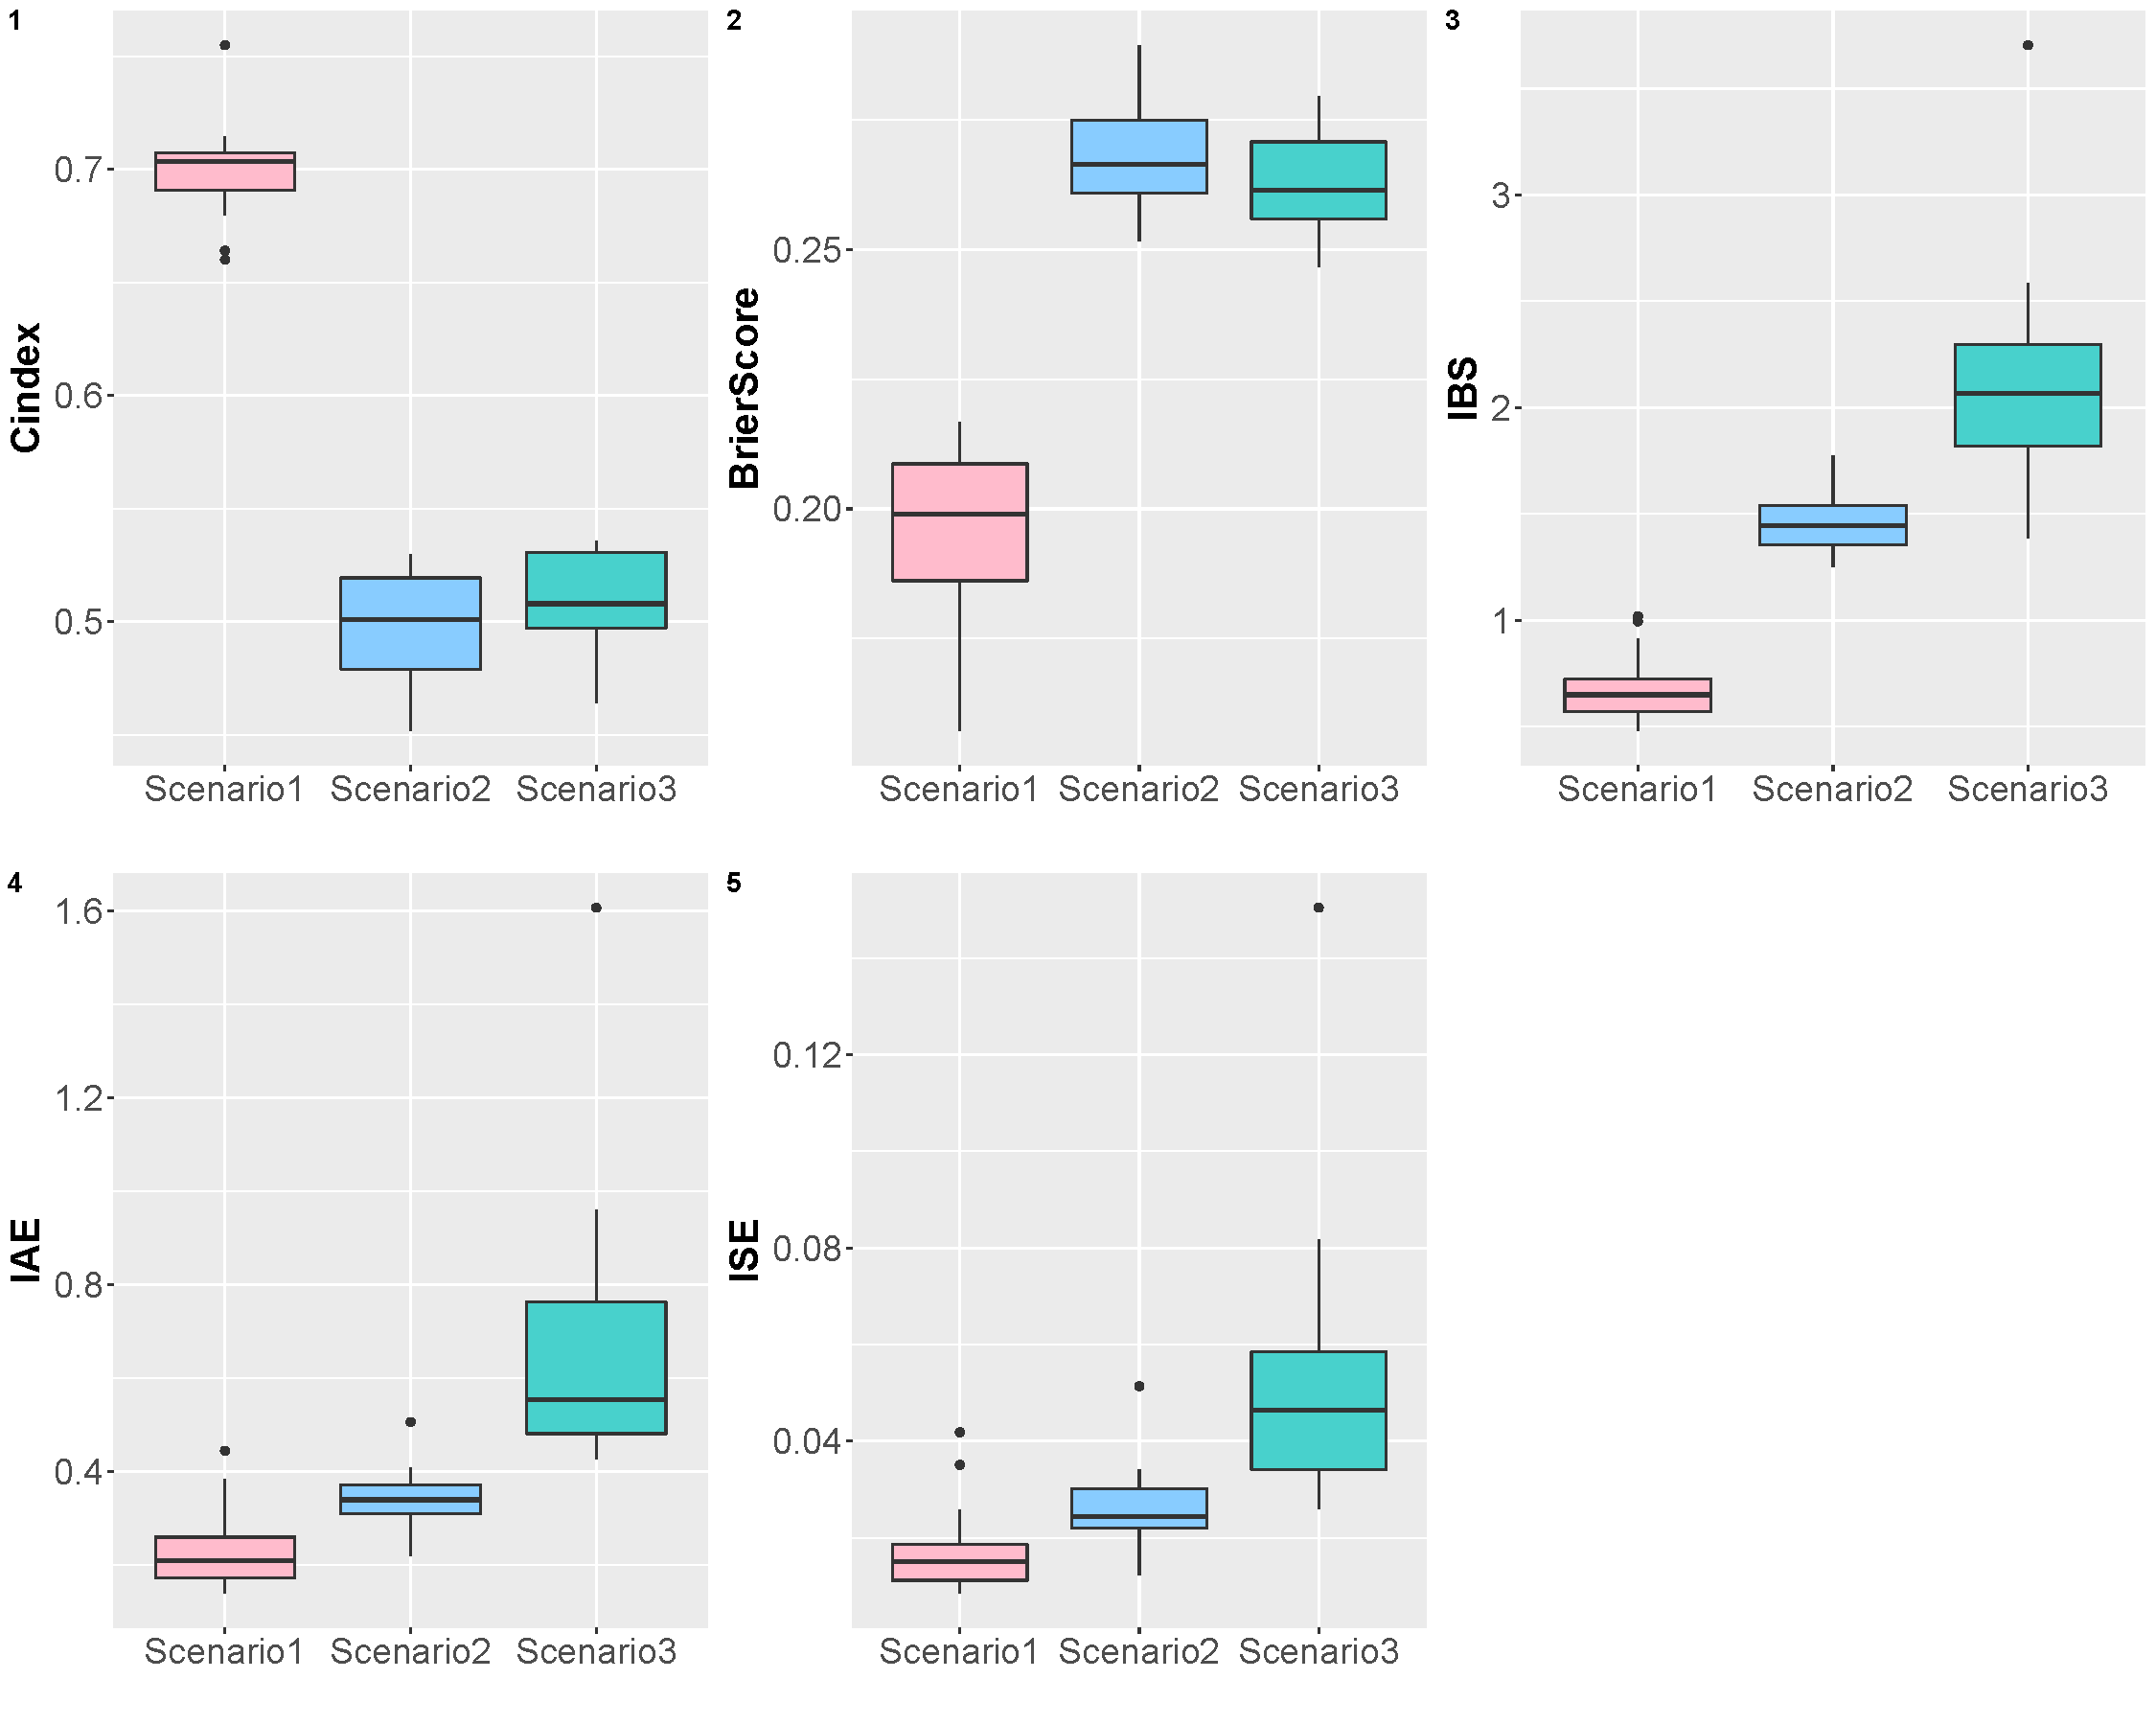
\includegraphics[width=\textwidth]{simuladataexp.pdf}
  \caption{
   This graphic shows the Cox model prediction accuracy based on three different scenarios via 5 evaluation metrics by the \pkg{SurvMetrics} package. The sample size is 300, the dimension is 25, and control the censoring rate about 30\%. The prediction performance of the Cox model keeps decreasing in three scenarios, which satisfies the data generated methods. However, in some complex situations where C-index and BS cannot distinguish models, IBS, IAE, and ISE, may be useful alternatives.}\label{fig3.1}
  \end{center}
\end{figure}


From Figure \ref{fig3.1}, one may see that the prediction performance of the Cox model keeps decreasing in three scenarios as expected. However, the difference in terms of C-index and BS are not significant for Scenario2 and Scenario3 while in terms of IBS, IAE and ISE, a sharp difference and a clear trend can be observed.

As we know, C-index evaluates the model from a ranking perspective in a rough matter and BS only considers a fixed time point. Both metrics may not distinguish models described above or in other complex settings. In this case, evaluation metrics which consider model performance in a global way, such as IBS, IAE, and ISE,  may be useful alternatives. This also justifies why a package such as \pkg{SurvMetrics} that can evaluate survival models from multiple perspectives is strongly needed in practice.


  \subsection{An example of \pkg{SurvMetrics}}\label{sec3.2}

  In this section, a kidney dataset from the \pkg{survival} R package is used to illustrate the usage of the \pkg{SurvMetrics} package using popular survival models widely used in biostatics and biomedical study.

  In the following, we first cut the kidney dataset into a training set and a testing set. Then, two popular models, namely, Cox model and random survival forest model are constructed based on the training set to show how different functions are used in \pkg{SurvMetrics}. Finally, we will show how to evaluate the predictive performance of these two models on the testing set using the proposed \pkg{SurvMetrics} R package.  In the latest version of \pkg{SurvMetrics}, user has the choice to input only the standard survival models and testing sets. Meanwhile, it is still useful to deal with predicted survival probabilities from non-standard models. The following example will contain these two input forms.

  The corresponding R code is provided here:

    %R code

\begin{example}
  #1. data preparation
  library(survival)        # to fit a Cox model
  library(randomForestSRC) # to fit an RSF model
  library(SurvMetrics) # to get all the metrics
  library(pec)         # to make predictions based on Cox model
  set.seed(1)
  mydata <- kidney[, -1]
  train_index <- sample(1:nrow(mydata), 0.7 * nrow(mydata))
  train_data <- mydata[train_index, ]
  test_data <- mydata[-train_index, ]

  #2. fit the RSF model and Cox model to predict the testing set
  #2.1 RSF model
  fit_rsf <- rfsrc(Surv(time,status)~., data = train_data)  #fit the RSF model
  distime <- fit_rsf$time.interest  #get the survival time of events
  med_index <- median(1:length(distime))  #the index of median survival time of events
  mat_rsf <- predict(fit_rsf, test_data)$survival  #get the survival probability matrix
  vec_rsf <- mat_rsf[ ,med_index]  #median survival probability of all samples

  #2.2 Cox model
  fit_cox <- coxph(Surv(time,status)~., data = train_data, x = TRUE)  #fit the Cox model
  mat_cox <- predictSurvProb(fit_cox, test_data, distime)  #get the survival probability matrix
  vec_cox <- mat_cox[ ,med_index]

  #3. get all the metrics by SurvMetrics
  #3.1 CI BS IBS IAE ISE based on RSF model: standard model input methods
  Cindex_rsf <- Cindex(fit_rsf, test_data)
  BS_rsf <- Brier(fit_rsf, test_data, distime[med_index])
  IBS_rsf <- IBS(fit_rsf, test_data)
  IAE_rsf <- IAEISE(fit_rsf, test_data)[1]
  ISE_rsf <- IAEISE(fit_rsf, test_data)[2]

  #CI BS IBS IAE ISE based on Cox model: standard model input methods
  Cindex_cox <- Cindex(fit_cox, test_data)
  BS_cox <- Brier(fit_cox, test_data, distime[med_index])
  IBS_cox <- IBS(fit_cox, test_data)
  IAE_cox <- IAEISE(fit_cox, test_data)[1]
  ISE_cox <- IAEISE(fit_cox, test_data)[2]

  #3.2 CI BS IBS IAE ISE based on RSF model: Non-standard model input methods
  times <- test_data$time
  status <- test_data$status
  Cindex_rsf <- Cindex(Surv(times, status), vec_rsf)
  BS_rsf <- Brier(Surv(times, status), vec_rsf, distime[med_index])
  IBS_rsf <- IBS(Surv(times, status), mat_rsf, distime)  # distime can be replaced by range(distime)
  IAE_rsf <- IAEISE(Surv(times, status), mat_rsf, distime)[1]
  ISE_rsf <- IAEISE(Surv(times, status), mat_rsf, distime)[2]

  #CI BS IBS IAE ISE based on Cox model: Non-standard model input methods
  Cindex_cox <- Cindex(Surv(times, status), vec_cox)
  BS_cox <- Brier(Surv(times, status), vec_cox, distime[med_index])
  IBS_cox <- IBS(Surv(times, status), mat_cox, distime)
  IAE_cox <- IAEISE(Surv(times, status), mat_cox, distime)[1]
  ISE_cox <- IAEISE(Surv(times, status), mat_cox, distime)[2]
\end{example}


\begin{table}[h]
  \centering
  \begin{tabular}{lccccc}
  \hline
  models & C-index  & BS       & IBS      & IAE      & ISE      \\
  \hline
  Cox    & 0.751185 & 0.18133  & 0.08842 & 77.90947 & 19.65131 \\
  RSF    & 0.729858 & 0.221523 & 0.10920 & 105.6936 & 28.80941\\
  \hline
  \end{tabular}
  \caption{
    This table shows the prediction accuracy by using \pkg{SurvMetrics} package to compare the Cox and RSF models based on the kidney data set from \pkg{survival} R package. In this case, the values of C-index are close, and the values of IAE and ISE are far different. When using C-index alone is hard to differentiate the predictive power of the two models, alternative measures provided in \pkg{SurvMetrics} may help give a more accurate result.}\label{tab3.2}
\end{table}

\begin{figure}[h]
  \centering
  \begin{center}
  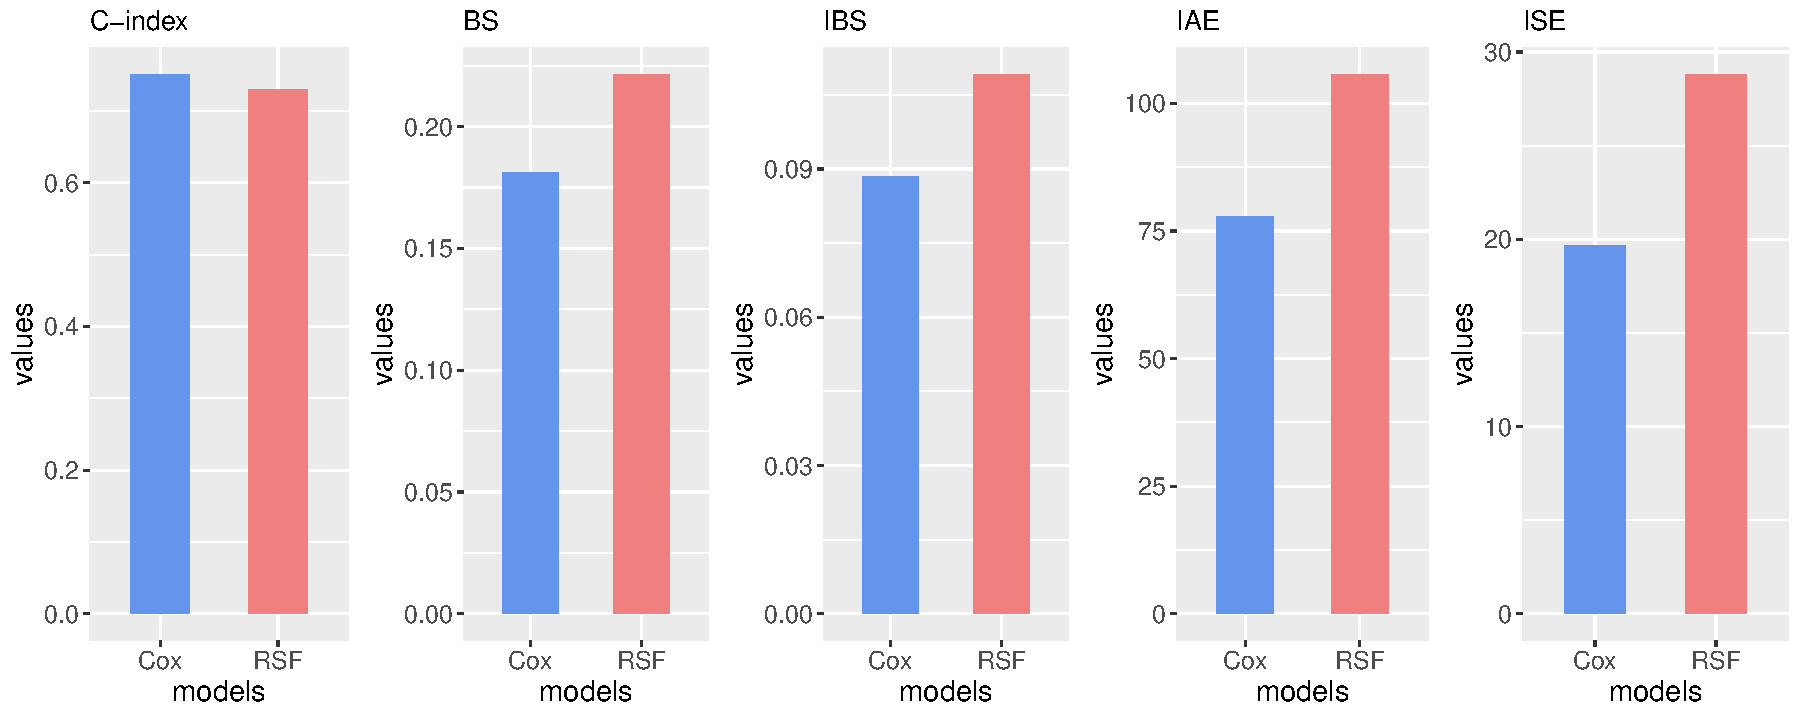
\includegraphics[width=\textwidth]{kidneyres.pdf}
  \caption{
    This graphic shows the prediction accuracy by using \pkg{SurvMetrics} package to compare the Cox and RSF models based on the kidney data set from \pkg{survival} R package. In this case, using IBS, IAE and ISE can give a more clear conclusion that Cox model performs better.}\label{fig3.2}
  \end{center}
\end{figure}

The results presented in Table \ref{tab3.2} and Figure \ref{fig3.2} show that using C-index alone is hard to differentiate the predictive power of the two models. In this case, alternative measures provided in the proposed package may help if further evaluation is needed. This result is also  consistent with the simulated scenario mentioned above.

\section{Summary}

Assessing the predictive performance of survival models is complex due to the lack of standards regarding the best criterion to use in survival analysis. The available metrics are scatter across different R packages that use heterogeneous interfaces, which makes it difficult for the non-specialist to  use or compare the performance of various survival models.

In this paper, we try to fill the gap by providing an "all-in-one" R package called \pkg{SurvMetrics} which provides a uniform interface to an extensive set of performance assessment and statistical comparison methods. Practitioners can easily implement comparative studies and identify the best model(s) using this package. In the current version of the \pkg{SurvMetrics} package, six  evaluation metrics are present. Evaluation metrics used in more complicated settings such as time-dependent AUC for joint modelling of longitudinal and survival data, and concordance index for competitive risks are still being developed and will be added to the \pkg{SurvMetrics}  package in the future. Meanwhile, we are also working to provide a more user-friendly interface to facilitate both statistical and non-statistical clinical research workers in evaluating survival models.

\section{Acknowledgments}
%This was partly supported by National Statistical Scientific Research Project of China (No.2022LZ28), Changsha Municipal Natural Science Foundation (No.kq2202080), Guangdong Provincial Key Laboratory of Big Data Computing, The Chinese University of Hong Kong, Shenzhen and the Postgraduate Scientific Research Innovation Project of Hunan Province, China (CX20210155).
This research is support in part by National Statistical Scientific Research Project of China (No.2022LZ28), Changsha Municipal Natural Science Foundation (No.kq2202080), The Open Research Fund from the Guangdong Provincial Key Laboratory of Big Data Computing, The Chinese University of Hong Kong, Shenzhen(No. B10120210117-OF04) and the Postgraduate Scientific Research Innovation Project of Hunan Province, China (CX20210155).

\bibliography{hanpu-zhou.bib}

%\section{Another section}
%
%This section may contain a figure such as Figure~\ref{figure:rlogo}.
%
%\begin{figure}[htbp]
%  \centering
%  
\includegraphics{Rlogo-5}
%  \caption{The logo of R.}
%  \label{figure:rlogo}
%\end{figure}
%
%\section{Another section}
%
%There will likely be several sections, perhaps including code snippets, such as:
%
%\begin{example}
%  x <- 1:10
%  result <- myFunction(x)
%\end{example}
%
%\section{Summary}
%
%This file is only a basic article template. For full details of \emph{The R Journal} style and information on how to prepare your article for submission, see the \href{https://journal.r-project.org/share/author-guide.pdf}{Instructions for Authors}.



\address{Hanpu Zhou\\
  Central South University\\
    School of Mathematics \& Statistics\\
    Changsha, Hunan Provinice,410075\\
    China\\
  \email{zhouhanpu@csu.edu.cn}}

\address{Hong Wang* \\
  Central South University\\
    School of Mathematics \& Statistics\\
    Changsha, Hunan Provinice,410075\\
    China\\
  (Corresponding Author)\\
  \email{wh@csu.edu.cn}}



\address{Sizheng Wang\\
    Central South University\\
    School of Mathematics \& Statistics\\
    Changsha, Hunan Provinice,410075\\
    China\\
    \email{wszhchina@163.com}}

\address{Yi Zou\\
Central South University\\
    School of Mathematics \& Statistics\\
    Changsha, Hunan Provinice,410075\\
    China\\
  \email{zy6868@csu.edu.cn}} 
  
  